\documentclass[11pt,a4paper]{article}

% ---- Mathematics (loaded before xepersian) ----
\usepackage{amsmath}
\usepackage{amssymb}
\usepackage{amsthm}
\usepackage{mathtools}

% ---- Layout ----
\usepackage[a4paper,left=1in,right=1in,top=1in,bottom=1in]{geometry}
\usepackage{graphicx}
\graphicspath{{../images/examples/}}
\usepackage{booktabs}
\usepackage{enumitem}
\usepackage{caption}
\usepackage{subcaption}
\captionsetup{font=small,labelfont=bf}
\usepackage{xcolor}
\usepackage[colorlinks=true,urlcolor=blue!50!black,linkcolor=blue!50!black,citecolor=blue!50!black]{hyperref}

% ---- Persian (xepersian must be loaded last) ----
% Main Persian text: XB Niloofar -- a free (OFL), academic, B Nazanin-style
% Naskh face with full diacritic coverage, ships Regular/Bold/Italic.
% Latin tokens and code use Latin Modern (matching the English article / maths).
\usepackage{xepersian}
\settextfont[Scale=1.05]{XB Niloofar}
\setlatintextfont{Latin Modern Roman}
\setmonofont{Latin Modern Mono}
\newfontfamily\enfont{Latin Modern Roman}
\newcommand{\en}[1]{\lr{{\enfont #1}}}

\hypersetup{
  pdftitle={Edge-Magic Total Labelings on G(m,n,k,t) -- Persian},
  pdfauthor={Bardia Yaghmaie}
}

% ---- Convenience macros ----
\newcommand{\Z}{\mathbb{Z}}
\newcommand{\km}{\kappa}
\newcommand{\Gfam}{G(m,n,k,t)}
\DeclareMathOperator{\AllDiff}{AllDifferent}
\DeclareMathOperator{\degr}{deg}

% ---- Persian theorem environments ----
\theoremstyle{plain}
\newtheorem{theorem}{قضیه}
\newtheorem{proposition}{گزاره}
\newtheorem{corollary}{نتیجه}
\newtheorem{lemma}{لم}
\theoremstyle{definition}
\newtheorem{definition}{تعریف}
\newtheorem{example}{مثال}
\theoremstyle{remark}
\newtheorem*{remark}{ملاحظه}
\renewcommand{\proofname}{اثبات}

\title{\textbf{برچسب‌گذاری جادویی کلِ یال‌ها روی خانوادهٔ گراف‌های\\ چهاربخشیِ $G(m,n,k,t)$}}

\author{
  بردیا یغمایی\\[2pt]
  \small دانشکده ریاضی و علوم کامپیوتر،\\
  \small دانشگاه علم و صنعت ایران، تهران، ایران\\
  \small \en{\href{mailto:bardia_yaghmaie@mathdep.iust.ac.ir}{bardia\_yaghmaie@mathdep.iust.ac.ir}} $\cdot$ \en{\href{mailto:yaghmaiebardia@gmail.com}{yaghmaiebardia@gmail.com}}
}

\date{بهمن ۱۴۰۴}

\begin{document}
\maketitle

\begin{abstract}
\noindent
یک \emph{برچسب‌گذاری جادویی کلِ یال‌ها} (به اختصار \en{EMTL}) از یک گراف سادهٔ متناهی
$G=(V,E)$ یک تناظر دوسویی $f\colon V\cup E\to\{1,2,\dots,|V|+|E|\}$ است که برای آن
ثابتی مانند $\km$ وجود دارد به‌طوری‌که برای هر یال $uv\in E$ رابطهٔ
$f(u)+f(uv)+f(v)=\km$ برقرار باشد. هیچ الگوریتمِ کارآمدِ عمومی برای تشخیصِ وجودِ چنین
برچسب‌گذاری‌ای شناخته نشده است و ساخت‌های صریح تنها برای رده‌های محدودی از
گراف‌ها به‌دست آمده‌اند. در این مقاله \en{EMTL} را روی یک خانوادهٔ پارامتری از
گراف‌های چهاربخشیِ $\Gfam$ مطالعه می‌کنیم؛ این گراف‌ها از دو لایهٔ دوبخشیِ کامل ساخته
می‌شوند که با یک لایهٔ میانیِ $t$-منتظمِ دوری به هم متصل شده‌اند. ما این خانواده را
صورت‌بندی می‌کنیم، یک اتحاد وزن‌دار بر حسب درجه به‌همراه یک شرط بخش‌پذیری و کران‌های
سراسری برای ثابت جادویی استخراج می‌کنیم، و یک \emph{تحویلِ تعیین‌شدگی توسط رأس‌ها} را
اثبات می‌کنیم که نشان می‌دهد به‌محض انتخابِ برچسبِ رأس‌ها و مقدار $\km$، کلِ
برچسب‌گذاری معین می‌شود. بر پایهٔ این نتایج، مسئلهٔ وجودِ \en{EMTL} را به‌صورت یک
مسئلهٔ ارضای قیود بیان کرده و آن را به‌طور دقیق با حل‌کنندهٔ \en{CP-SAT} از مجموعهٔ
\en{OR-Tools} حل می‌کنیم؛ این حل‌کننده یا یک برچسب‌گذاریِ تأییدشده بازمی‌گرداند، یا
گواهیِ ناممکن‌بودن می‌دهد، یا اعلام اتمام زمان می‌کند. آزمایش‌هایی را برای بازه‌ای از
پارامترها گزارش می‌کنیم و یک پیاده‌سازیِ مرجعِ متن‌بازِ همراه با مجموعه‌آزمون و
ابزار ترسیم ارائه می‌دهیم.

\medskip
\noindent\textbf{واژگان کلیدی:} برچسب‌گذاری جادویی کلِ یال‌ها، برچسب‌گذاری گراف،
برنامه‌ریزی با قید، \en{CP-SAT}، گراف‌های چهاربخشی.
\end{abstract}

\section{مقدمه}\label{sec:intro}

یک \emph{برچسب‌گذاری گراف} اعدادی را به رأس‌ها و/یا یال‌های یک گراف، تحت شرایطی
ساختاری، نسبت می‌دهد؛ خاستگاه این حوزه به کارِ کوتزیگ و روزا دربارهٔ \emph{ارزش‌گذاری‌های
جادویی}~\cite{kotzig-rosa} بازمی‌گردد و گونه‌های بسیاری که از آن پس مطالعه شده‌اند در
پیمایش پویای گالیان~\cite{gallian} و کتابِ والیس~\cite{wallis} فهرست شده‌اند. در یک
\emph{برچسب‌گذاری جادویی کلِ یال‌ها} هر عددِ مجموعهٔ $\{1,\dots,|V|+|E|\}$ دقیقاً یک‌بار
در میان همهٔ رأس‌ها و یال‌ها به‌کار می‌رود (یک تناظر دوسوییِ سراسری)، و هم‌زمان هر یال
به یک مجموعِ القاییِ یکسان وادار می‌شود (یک معادلهٔ موضعی). برهم‌کنشِ این دو شرط است
که مسئله را ظریف می‌کند: هیچ الگوریتمِ زمان-چندجمله‌ای برای مسئلهٔ عمومی شناخته نشده
است و بیشترِ نتایجِ مثبت به‌شکلِ ساخت‌های صریح برای رده‌های خاصی از گراف‌ها مانند دورها،
مسیرها، گراف‌های دوبخشیِ کامل و کتاب‌ها ظاهر می‌شوند~\cite{kotzig-rosa,wbms,gallian,kite}.

این مقاله دیدگاهی مکمّل، محاسباتی و مختص‌خانواده اتخاذ می‌کند. ما یک خانوادهٔ
ساختارمند از گراف‌های چهاربخشیِ $\Gfam$ را تثبیت می‌کنیم که به‌قدر کافی غنی هست که
جالب باشد و در عین حال به‌قدر کافی منظم است که آزمایشِ نظام‌مند را ممکن سازد، و وجودِ
\en{EMTL} را روی این خانواده به‌طور \emph{دقیق} با برنامه‌ریزی با قید بررسی می‌کنیم.
به‌طور مشخص، دستاوردها چنین‌اند:

\begin{enumerate}[label=(\arabic*),itemsep=1pt]
  \item تعریفی دقیق از خانوادهٔ گراف $\Gfam$ و ناورداهای ساختاریِ پایهٔ آن
        (بخش~\ref{sec:family})؛
  \item شرایطِ \emph{لازمِ} جبری برای یک \en{EMTL} از $\Gfam$ --- یک اتحادِ وزن‌دار بر
        حسبِ درجه، یک شرطِ بخش‌پذیری/همنهشتی، و کران‌های سراسری برای ثابت جادویی
        (بخش~\ref{sec:algebra})؛
  \item یک \emph{تحویلِ تعیین‌شدگی توسط رأس‌ها}: به‌محضِ انتخابِ ثابت جادویی و برچسبِ
        رأس‌ها، همهٔ برچسب‌های یال معین می‌شوند (گزاره~\ref{prop:reduction})، که هم
        فضای جست‌وجو را روشن می‌کند و هم مدلِ قیدی را فشرده‌تر می‌سازد
        (بخش~\ref{sec:model})؛
  \item یک صورت‌بندیِ دقیقِ \en{CP-SAT} و یک پیاده‌سازیِ مرجعِ متن‌باز، به‌همراه یک
        مطالعهٔ آزمایشی در بازه‌های گوناگونِ پارامتر
        (بخش‌های~\ref{sec:model}--\ref{sec:experiments}).
\end{enumerate}

شرایطِ لازم برای \emph{تصمیم‌گیری} دربارهٔ نمونه‌ها به‌کار نمی‌روند --- این کار را
حل‌کننده انجام می‌دهد --- بلکه به‌عنوانِ کرانِ حل‌کننده و ناوردای مستقلِ صحت پس از حل
عمل می‌کنند و توضیح می‌دهند که چرا ثابت جادویی را نمی‌توان آزادانه انتخاب کرد.

\section{مقدمات}\label{sec:prelim}

در سراسرِ مقاله، $G=(V,E)$ یک گرافِ سادهٔ متناهیِ بدون‌جهت است،
$N:=|V|+|E|$، و $\degr(v)$ درجهٔ رأسِ $v$ را نشان می‌دهد.

\begin{definition}[برچسب‌گذاری کل]
یک \emph{برچسب‌گذاری کل} از $G$ تابعی است $f\colon V\cup E\to\{1,2,\dots,N\}$. این
برچسب‌گذاری \emph{دوسویی} است اگر یک‌به‌یک و پوشا باشد؛ به‌طور معادل، چندمجموعهٔ
برچسب‌های نسبت‌داده‌شده دقیقاً برابرِ $\{1,2,\dots,N\}$ باشد.
\end{definition}

\begin{definition}[برچسب‌گذاری جادویی کلِ یال‌ها]\label{def:emtl}
یک برچسب‌گذاری کلِ دوسویی $f$ یک \emph{برچسب‌گذاری جادویی کلِ یال‌ها} (\en{EMTL})
است اگر ثابتی مانند $\km\in\Z$ وجود داشته باشد که
\[
  f(u)+f(uv)+f(v)=\km \qquad\text{برای هر یال } uv\in E .
\]
ثابتِ $\km$ را \emph{ثابت جادویی} (یا \emph{مجموعِ جادویی}) می‌نامیم. گرافی که یک
\en{EMTL} می‌پذیرد \emph{یال‌جادویی} نامیده می‌شود.
\end{definition}

تحقیق ارزان است: با داشتنِ یک نامزدِ $(\km,f)$، دوسویی‌بودن و $|E|$ معادلهٔ یال در
زمانِ $O(N)$ بررسی می‌شوند. یافتنِ یک برچسب‌گذاری، یا گواهی‌کردنِ عدمِ وجودِ آن، جهتِ
دشوار است و موضوعِ این مقاله است.

\section{خانوادهٔ گراف \texorpdfstring{$G(m,n,k,t)$}{G(m,n,k,t)}}\label{sec:family}

\subsection{بخش‌بندیِ رأس‌ها و لایه‌های یال}

اعدادِ صحیحِ $m,n,k\ge 1$ و عددِ صحیحِ $t$ با $0\le t\le n$ را ثابت می‌گیریم. مجموعهٔ
رأس‌ها به چهار بخشِ مجزا افراز می‌شود:
\[
  A=\{A_0,\dots,A_{m-1}\},\quad
  B=\{B_0,\dots,B_{n-1}\},\quad
  C=\{C_0,\dots,C_{n-1}\},\quad
  D=\{D_0,\dots,D_{k-1}\},
\]
با $|A|=m$، $|B|=|C|=n$، $|D|=k$، به‌طوری‌که
\begin{equation}\label{eq:Vcount}
  |V| = m + 2n + k .
\end{equation}
مجموعهٔ یال‌ها اجتماعِ سه لایهٔ دوبخشی است:
\begin{enumerate}[label=(\arabic*),itemsep=1pt]
  \item لایهٔ \emph{چپِ} دوبخشیِ کاملِ $K_{m,n}$ میانِ $A$ و $B$ (هر $mn$ یال)؛
  \item لایهٔ \emph{میانیِ} $t$-منتظمِ دوبخشی میانِ $B$ و $C$ ($nt$ یال)؛
  \item لایهٔ \emph{راستِ} دوبخشیِ کاملِ $K_{n,k}$ میانِ $C$ و $D$ (هر $nk$ یال).
\end{enumerate}
بنابراین
\begin{equation}\label{eq:Ecount}
  |E| = mn + nt + nk .
\end{equation}

\begin{remark}\label{rem:boundary}
برای $t=0$ لایهٔ میانی تهی است و $\Gfam$ اجتماعِ مجزای $K_{m,n}\sqcup K_{n,k}$ می‌شود؛
\en{EMTL} روی یک گرافِ ناهمبند نیز تعریف‌شده است و تحلیلِ زیر بی‌تأثیر می‌ماند. در حدِ
دیگر، یعنی $t=n$، لایهٔ میانی همان گرافِ دوبخشیِ کاملِ $K_{n,n}$ است.
\end{remark}

\subsection{ساختِ دوریِ لایهٔ میانی}

لایهٔ میانی با قاعدهٔ دوریِ زیر ساخته می‌شود:
\begin{equation}\label{eq:circulant}
  E_{BC}=\bigl\{\, (B_i,\,C_{(i+j)\bmod n}) \;:\; i\in\{0,\dots,n-1\},\; j\in\{0,\dots,t-1\} \,\bigr\}.
\end{equation}

\begin{proposition}[منتظم‌بودنِ لایهٔ میانی]\label{prop:regular}
برای $0\le t\le n$، گرافِ دوبخشیِ $(B\cup C,\,E_{BC})$ در~\eqref{eq:circulant} از هر
دو سو $t$-منتظم است.
\end{proposition}

\begin{proof}
بنا بر~\eqref{eq:circulant}، $B_i$ با $C_{(i)\bmod n},\dots,C_{(i+t-1)\bmod n}$ مجاور
است. چون $t\le n$، $t$ باقی‌ماندهٔ متوالیِ $i,i+1,\dots,i+t-1 \pmod n$ دوبه‌دو متمایزند،
پس این‌ها $t$ همسایهٔ متمایزند --- و به‌ویژه لایه ساده است --- و درجهٔ $B_i$ برابرِ $t$
است. برعکس، $C_r$ را ثابت بگیرید. آن‌گاه $(B_i,C_r)\in E_{BC}$ اگر و تنها اگر برای
$j\in\{0,\dots,t-1\}$ ای داشته باشیم $r\equiv i+j\pmod n$، یعنی $i\equiv r-j\pmod n$؛
چون $t\le n$، این‌ها $t$ رأسِ متمایزِ $B_{(r)\bmod n},\dots,B_{(r-t+1)\bmod n}$ هستند.
پس درجهٔ $C_r$ نیز $t$ است.
\end{proof}

\begin{proposition}[دنبالهٔ درجه‌ها]\label{prop:degrees}
در $\Gfam$ درجه روی هر بخش ثابت است:
\[
  \degr(a)=n \ (a\in A),\quad
  \degr(b)=m+t \ (b\in B),\quad
  \degr(c)=k+t \ (c\in C),\quad
  \degr(d)=n \ (d\in D).
\]
\end{proposition}

\begin{proof}
هر $a\in A$ تنها به همهٔ $B$ متصل است و به چیزِ دیگری نه، پس $\degr(a)=n$؛ به‌تقارن
$\degr(d)=n$. هر $b\in B$ به همهٔ $A$ ($m$ یال) و، بنا بر گزاره~\ref{prop:regular}، به
$t$ رأس از $C$ متصل است، پس $\degr(b)=m+t$؛ به‌تقارن $\degr(c)=k+t$.
\end{proof}

\noindent
شکل~\ref{fig:structure} یک نمونهٔ کوچک را با سه لایه و یک برچسب‌گذاریِ یافت‌شده
نشان می‌دهد.

\begin{figure}[t]
  \centering
  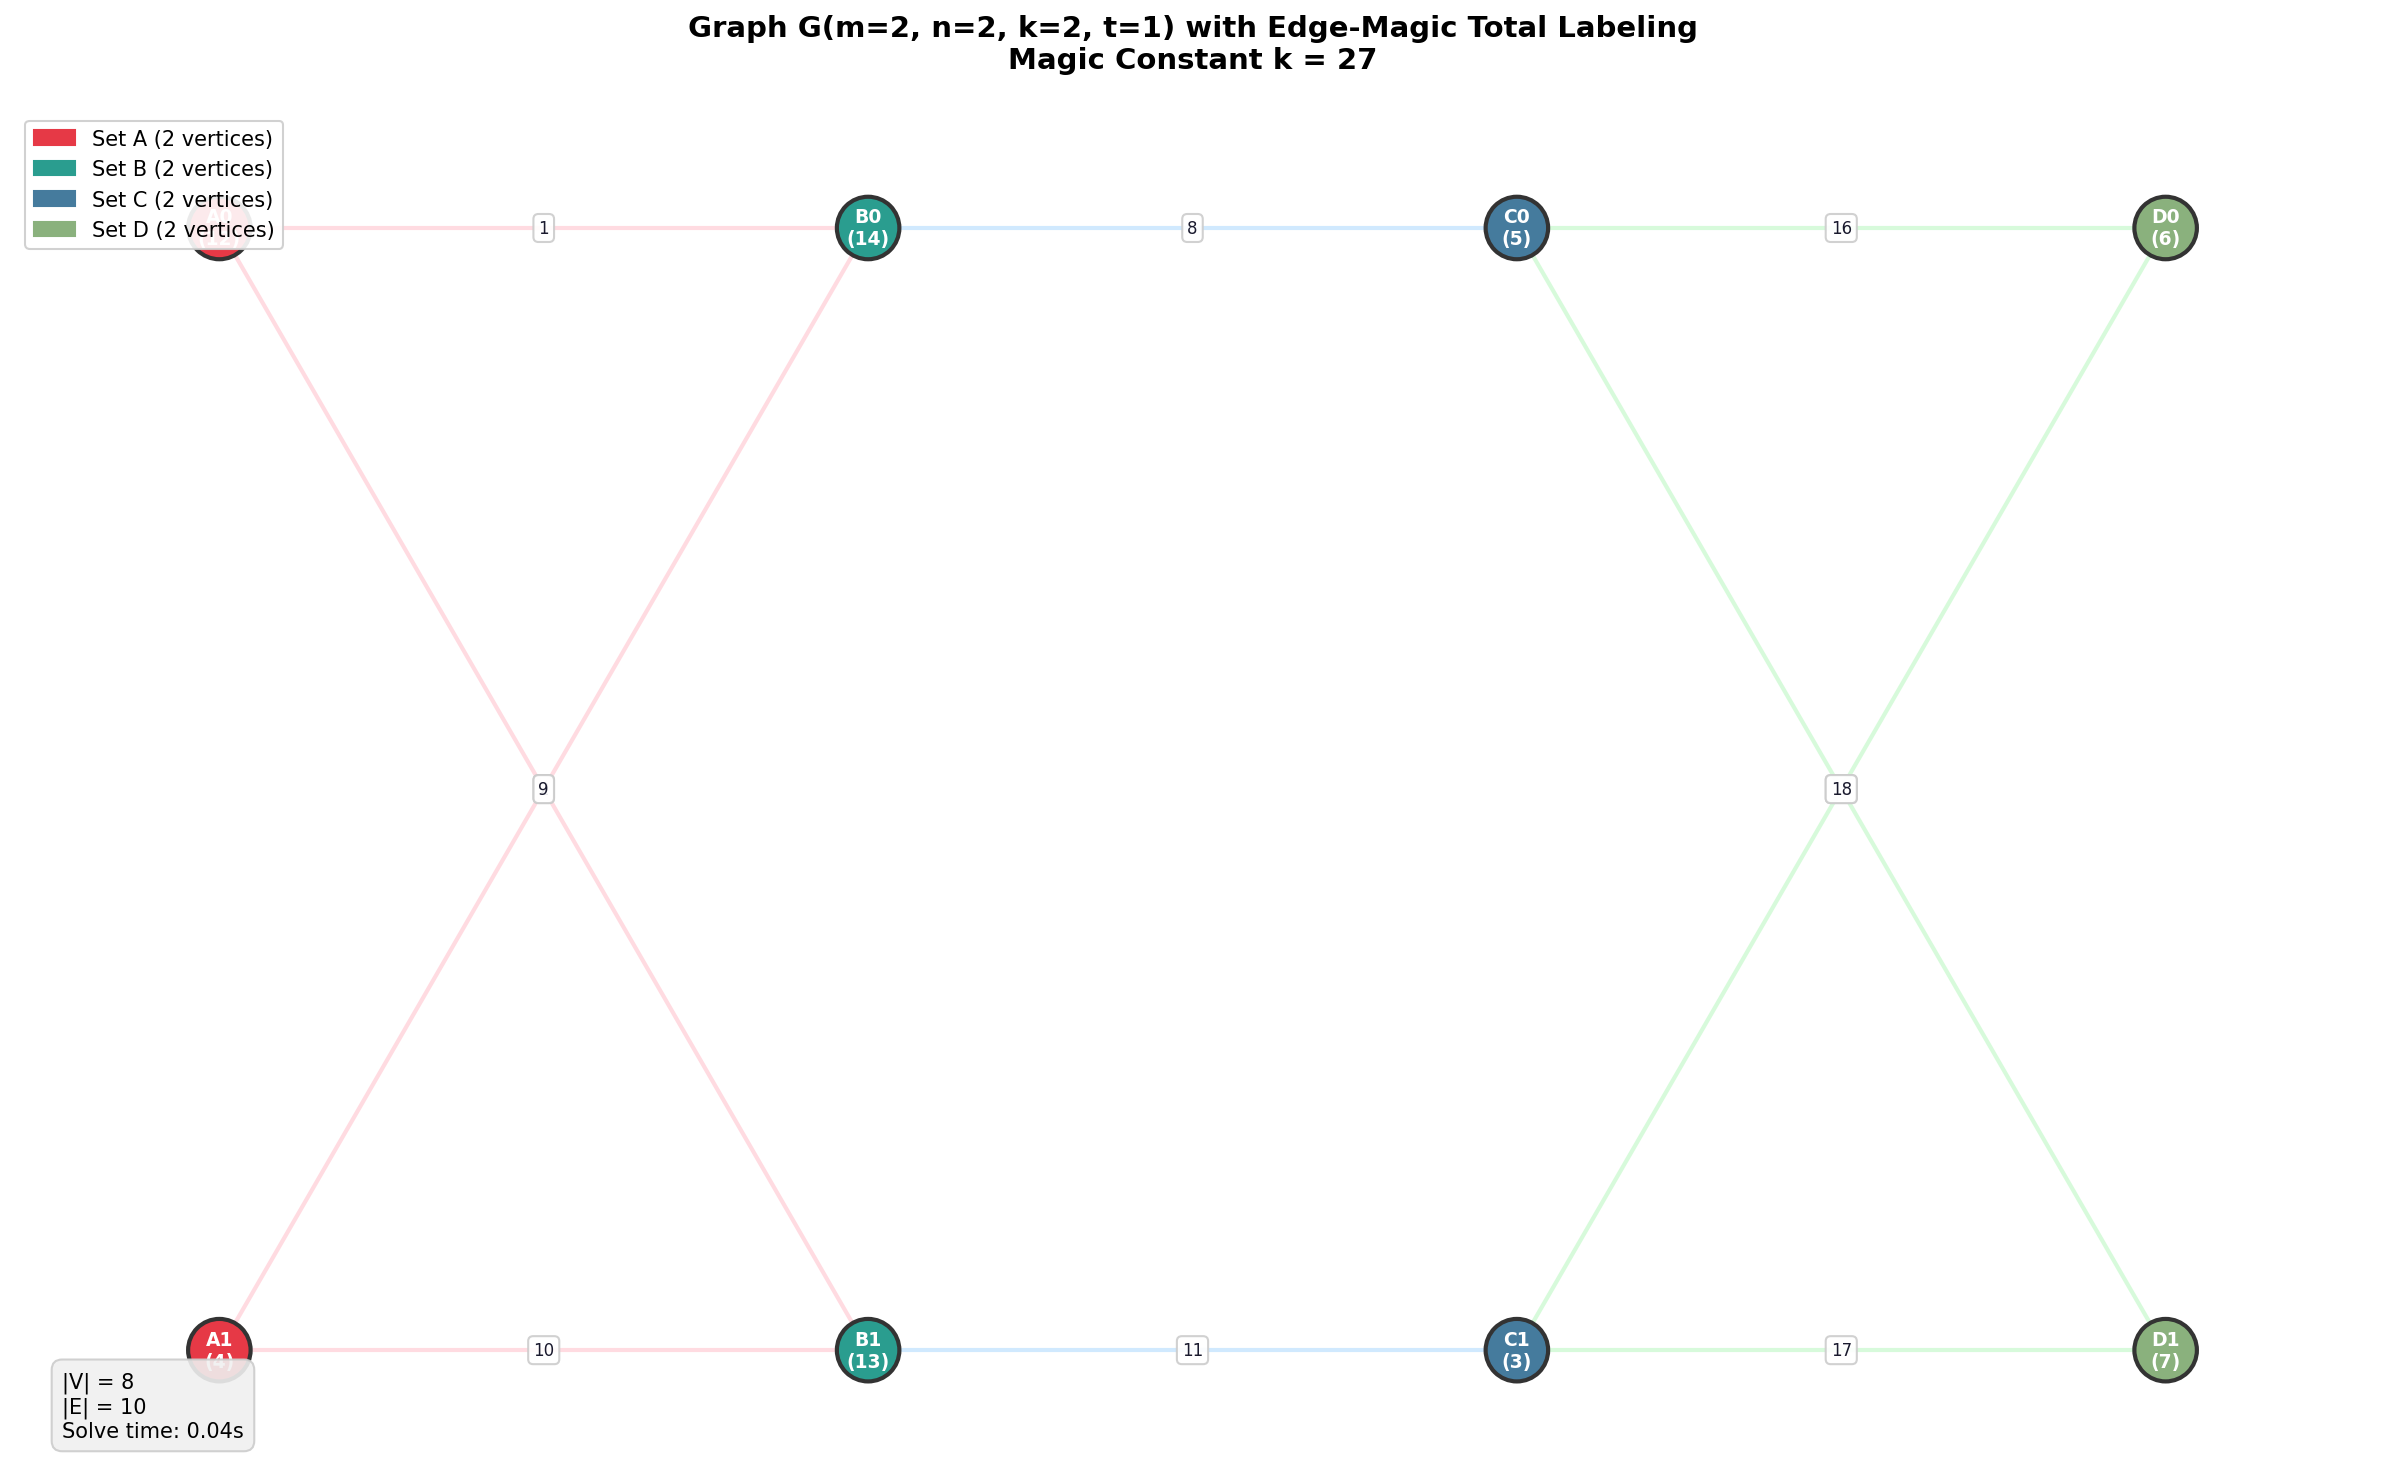
\includegraphics[width=0.82\textwidth]{emtl_m2_n2_k2_t1.png}
  \caption{گرافِ $G(2,2,2,1)$ با چهار بخشِ $A,B,C,D$ (از چپ به راست)، دو لایهٔ
  دوبخشیِ کاملِ $K_{2,2}$ (یعنی $A$--$B$ و $C$--$D$) و لایهٔ میانیِ $1$-منتظم
  ($B$--$C$). برچسب‌های رأس و یالِ یک \en{EMTL}ِ محاسبه‌شده نمایش داده شده‌اند؛ مجموعِ
  هر یال برابرِ ثابت جادویی $\km$ است.}
  \label{fig:structure}
\end{figure}

\section{شرایطِ لازمِ جبری}\label{sec:algebra}

این بخش اتحادهایی را ثبت می‌کند که هر \en{EMTL} از $G$ باید برآورده کند. این‌ها برای
\emph{حلِ} یک نمونه لازم نیستند، اما ثابت جادویی را مقید می‌کنند، کران‌های جست‌وجوی
مورد استفادهٔ حل‌کننده را فراهم می‌آورند و به‌عنوان بررسی‌های مستقلِ پس از حل عمل
می‌کنند.

فرض کنید $f$ یک \en{EMTL} از $G=(V,E)$ با ثابت جادویی $\km$ باشد. با جمع‌بستنِ معادلهٔ
جادوییِ تعریف~\ref{def:emtl} روی همهٔ یال‌ها داریم:
\begin{equation}\label{eq:sum0}
  \sum_{uv\in E}\bigl(f(u)+f(uv)+f(v)\bigr) = |E|\,\km .
\end{equation}

\begin{lemma}[مجموعِ سرها به‌صورتِ مجموعِ وزن‌دارِ رأس‌ها]\label{lem:endpoint}
$\displaystyle \sum_{uv\in E}\bigl(f(u)+f(v)\bigr)=\sum_{v\in V}\degr(v)\,f(v).$
\end{lemma}

\begin{proof}
مجموعِ مضاعف را بر حسبِ رأس‌ها بازچینی می‌کنیم: هر برچسبِ $f(v)$ به‌ازای هر یالِ مجاورِ
$v$ که تعدادشان $\degr(v)$ است، یک‌بار شمرده می‌شود، پس
\[
  \sum_{uv\in E}\bigl(f(u)+f(v)\bigr)
   =\sum_{v\in V} f(v)\,\bigl|\{e\in E: v\in e\}\bigr|
   =\sum_{v\in V}\degr(v)\,f(v).
\]
\end{proof}

\begin{proposition}[اتحادِ وزن‌دار بر حسبِ درجه]\label{prop:identity}
قرار دهید $S_N:=\sum_{i=1}^{N} i=\tfrac{N(N+1)}{2}$. هر \en{EMTL} از $G$ در رابطهٔ زیر
صدق می‌کند:
\begin{equation}\label{eq:identity}
  |E|\,\km \;=\; S_N \;+\; \sum_{v\in V}\bigl(\degr(v)-1\bigr) f(v).
\end{equation}
\end{proposition}

\begin{proof}
رابطهٔ~\eqref{eq:sum0} را به سهمِ یال‌ها و سهمِ رأس‌ها تفکیک کرده و
لم~\ref{lem:endpoint} را به‌کار می‌بریم:
\[
  |E|\,\km=\sum_{e\in E}f(e)+\sum_{v\in V}\degr(v)f(v).
\]
چون $f$ یک تناظرِ دوسویی روی $\{1,\dots,N\}$ است، داریم
$\sum_{e\in E}f(e)+\sum_{v\in V}f(v)=S_N$، پس
$\sum_{e\in E}f(e)=S_N-\sum_{v\in V}f(v)$. جای‌گذاری،~\eqref{eq:identity} را می‌دهد.
\end{proof}

\begin{remark}
برای $\Gfam$، ضریبِ $\degr(v)-1$ تنها مقادیرِ $n-1$ (روی $A$ و $D$)، $m+t-1$ (روی $B$)
و $k+t-1$ (روی $C$) را می‌گیرد، بنا بر گزاره~\ref{prop:degrees}.
\end{remark}

\begin{corollary}[شرطِ بخش‌پذیری/همنهشتی]\label{cor:divis}
با نمادگذاریِ گزاره~\ref{prop:identity}،
\[
  \km=\frac{S_N+\sum_{v\in V}(\degr(v)-1)f(v)}{|E|},
  \qquad\text{پس}\qquad
  S_N+\sum_{v\in V}(\degr(v)-1)f(v)\equiv 0 \pmod{|E|}.
\]
به‌ویژه، صورتِ کسر باید بر $|E|$ بخش‌پذیر باشد. این شرط لازم است اما برای وجودِ یک
\en{EMTL} کافی نیست.
\end{corollary}

\begin{proposition}[کران‌های سراسری برای ثابت جادویی]\label{prop:bounds}
هر \en{EMTL} در $\;6\le \km\le 3N-3\;$ صدق می‌کند.
\end{proposition}

\begin{proof}
روی یک یالِ $uv$، عناصرِ $u$، $uv$ و $v$ سه عضوِ متمایز از $V\cup E$ هستند، پس
برچسب‌هایشان متمایزند زیرا $f$ یک‌به‌یک است. هر مجموعِ سه برچسبِ متمایز از
$\{1,\dots,N\}$ دستِ‌کم $1+2+3=6$ و حداکثر $N+(N-1)+(N-2)=3N-3$ است؛ چون این برای هر
یال برقرار است، $\km$ نیز همین کران‌ها را دارد. (اینجا $N=|V|+|E|\ge 3$ است، زیرا $G$
دستِ‌کم یک یال دارد، پس بازه ناتهی است.)
\end{proof}

پیاده‌سازی از گزاره~\ref{prop:bounds} به‌عنوانِ دامنهٔ متغیرِ ثابت جادویی در مدلِ
قیدیِ بخش~\ref{sec:model} استفاده می‌کند.

\section{تحویل و مدلِ قیدی}\label{sec:model}

\subsection{تحویلِ تعیین‌شدگی توسط رأس‌ها}

معادلهٔ جادویی بر حسبِ برچسبِ یال تابعی است: با مرتب‌سازیِ دوبارهٔ تعریف~\ref{def:emtl}
به $f(uv)=\km-f(u)-f(v)$ می‌رسیم. این یک تحویلِ تمیز به‌دست می‌دهد.

\begin{proposition}[تعیین‌شدگی توسط رأس‌ها]\label{prop:reduction}
فرض کنید $G=(V,E)$ و یک ثابتِ $\km$ و یک تابعِ یک‌به‌یکِ
$x\colon V\to\{1,\dots,N\}$ را ثابت بگیرید. مقادیرِ القاییِ یال را با
$y_{uv}:=\km-x_u-x_v$ برای $uv\in E$ تعریف کنید. آن‌گاه $(\km,x)$ به یک \en{EMTL} از
$G$ گسترش می‌یابد اگر و تنها اگر:
\begin{enumerate}[label=(\alph*),itemsep=1pt]
  \item برای هر $uv\in E$، $y_{uv}\in\{1,\dots,N\}$؛
  \item مقادیرِ $\{y_{uv}:uv\in E\}$ دوبه‌دو متمایز باشند؛ و
  \item $\{y_{uv}:uv\in E\}\cap\{x_v:v\in V\}=\varnothing$.
\end{enumerate}
هرگاه این‌ها برقرار باشند، \en{EMTL} با داشتنِ $(\km,x)$ یکتاست، یعنی $f|_V=x$ و
$f(uv)=y_{uv}$.
\end{proposition}

\begin{proof}
اگر $f$ یک \en{EMTL} با $f|_V=x$ و ثابت جادویی $\km$ باشد، آن‌گاه معادلهٔ جادویی
$f(uv)=\km-x_u-x_v=y_{uv}$ را وادار می‌کند، پس برچسب‌های یال معین‌اند. چون $f$ یک تناظرِ
دوسویی روی $\{1,\dots,N\}$ است، هر مقدارِ یال در $y_{uv}\in\{1,\dots,N\}$ صدق می‌کند
(شرطِ (الف))، مقادیرِ $y_{uv}$ دوبه‌دو متمایزند (شرطِ (ب))، و هیچ $y_{uv}$ برابرِ برچسبِ
رأسی $x_v$ نیست (شرطِ (ج)). برعکس، اگر
(الف)--(ج) برقرار باشند، آن‌گاه $f$ با $f|_V=x$ و $f(uv)=y_{uv}$ مقادیری در
$\{1,\dots,N\}$ می‌گیرد، روی $V\cup E$ یک‌به‌یک است (رأس‌ها بنا بر فرض، یال‌ها بنا بر
(ب)، و دو مجموعه بنا بر (ج) متمایزند) و در نتیجه دوسویی است زیرا $|V\cup E|=N$. بنا بر
ساخت، در هر معادلهٔ جادویی صدق می‌کند.
\end{proof}

گزاره~\ref{prop:reduction} نشان می‌دهد که وجودِ \en{EMTL}، در اصل، یک جست‌وجو روی $\km$
و برچسب‌گذاریِ رأس‌ها به‌تنهایی است: برچسب‌های یال هرگز نیازی به حدس‌زدن ندارند.
حل‌کنندهٔ زیر برای وضوح و برای تحقیقِ مستقیم، متغیرهای صریحِ یال را نگه می‌دارد، اما
دقیقاً همین ساختار را به‌کار می‌گیرد --- تثبیتِ برچسبِ رأس‌ها برچسبِ یال‌ها را وادار
می‌کند، که آن‌گاه از طریقِ قیدِ دوسویی به‌شدت انتشار می‌یابد.

\subsection{صورت‌بندیِ CP-SAT}

ما وجودِ \en{EMTL} را به‌صورتِ یک مسئلهٔ ارضای قیود (بدون تابعِ هدف) مدل می‌کنیم. فرض
کنید $N=|V|+|E|$.

\paragraph{متغیرها.}
\begin{itemize}[itemsep=1pt]
  \item یک متغیرِ برچسبِ $x_v\in\{1,\dots,N\}$ برای هر رأسِ $v\in V$؛
  \item یک متغیرِ برچسبِ $x_e\in\{1,\dots,N\}$ برای هر یالِ $e\in E$ (وقتی $e=uv$، آن را
        $x_{uv}$ نیز می‌نویسیم)؛
  \item متغیرِ ثابت جادویی $\km\in\{6,\dots,3N-3\}$ (گزاره~\ref{prop:bounds}).
\end{itemize}

\paragraph{قیدها.}
\begin{align}
  &\AllDiff\bigl(\{x_v:v\in V\}\cup\{x_e:e\in E\}\bigr), \tag{C1}\label{eq:c1}\\
  &x_u+x_{uv}+x_v=\km \qquad\text{برای هر } uv\in E. \tag{C2}\label{eq:c2}
\end{align}
چون هر $N$ متغیرِ برچسب دامنهٔ مشترکِ $\{1,\dots,N\}$ را دارند، قیدِ \eqref{eq:c1}
آن‌ها را وادار می‌کند که یک تناظرِ دوسویی روی $\{1,\dots,N\}$ باشند؛ \eqref{eq:c2}
خاصیتِ جادویی است. بنابراین مدل $N+1$ متغیرِ صحیح، یک قیدِ تمایزِ کلی و $|E|$ معادلهٔ
خطی دارد. بنا بر \eqref{eq:Vcount}--\eqref{eq:Ecount} اندازهٔ مدل می‌تواند به‌صورتِ
مرتبهٔ دومی در پارامترها رشد کند --- تنها لایهٔ میانی $nt$ یال دارد، تا $n^2$ آن‌گاه که
$t=\Theta(n)$.

\subsection{چرا CP-SAT}\label{sub:whycpsat}

ما مدل را با \en{CP-SAT} از \en{OR-Tools}~\cite{ortools} حل می‌کنیم؛ این یک حل‌کنندهٔ
ترکیبی است که انتشارِ قید روی دامنه‌های صحیح را با یادگیریِ بندِ مبتنی بر تعارض به سبکِ
\en{SAT} درمی‌آمیزد. دو ویژگیِ مدلِ \en{EMTL} آن را گزینهٔ مناسبی می‌کنند. نخست، بنا بر
گزاره~\ref{prop:reduction}، هر معادلهٔ جادویی~\eqref{eq:c2} تابعی است، پس به‌محضِ
تثبیتِ دو برچسب از سه برچسبِ یک یال، برچسبِ سوم وادار می‌شود؛ بنابراین انتشار،
تخصیص‌های جزئیِ رأس‌ها را به برچسب‌های یالِ وادارشده تبدیل می‌کند. دوم، قیدِ تمایزِ
سراسری~\eqref{eq:c1} هر برچسب را به دیگری مقید می‌کند، پس یک مقدارِ وادارشدهٔ منفرد
می‌تواند دامنه‌های بسیاری را هرس کند، و بندهای تعارضِ آموخته‌شده مانع از آن می‌شوند که
جست‌وجو همان الگوهای ناممکن را دوباره کشف کند --- الگوهایی که فراوان‌اند، زیرا خانواده
زیرپیکربندی‌های ساختاریِ یکسانِ بسیاری دارد. هنگامی که جست‌وجو درختِ خود را بدونِ
یافتنِ جواب به پایان برساند، حل‌کننده به‌جای صرفِ اعلامِ اتمامِ زمان، یک گواهیِ راستینِ
ناممکن‌بودن بازمی‌گرداند.

\section{پیاده‌سازیِ مرجع}\label{sec:impl}

حل‌کننده با زبانِ پایتون (\en{\texttt{emtl\_solver.py}}) بر پایهٔ \en{networkx} و
\en{OR-Tools}، به‌همراه یک ابزارِ ترسیمِ \en{matplotlib} و یک رابطِ وبِ \en{Streamlit}،
پیاده‌سازی شده است. جدول~\ref{tab:impl} اشیای ریاضیِ این مقاله را به کُد نگاشت می‌دهد.
نقطهٔ ورودِ سرتاسریِ \en{\texttt{solve\_emtl(m,n,k,t,timeout)}} پارامترها را اعتبارسنجی
می‌کند، $\Gfam$ را می‌سازد، مدلِ بخش~\ref{sec:model} را ساخته و حل می‌کند، و هر
برچسب‌گذاریِ بازگردانده‌شده را به‌طور مستقل در برابرِ تعریف~\ref{def:emtl} تحقیق می‌کند.

\begin{table}[t]
  \centering
  \small
  \begin{tabular}{@{}ll@{}}
    \toprule
    \textbf{شیءِ ریاضی} & \textbf{کُد} \\
    \midrule
    پارامترهای $(m,n,k,t)$، شمارش‌های $|V|,|E|,N$ & \en{\texttt{GraphParameters}} \\
    گرافِ $\Gfam$ و لایهٔ دوریِ~\eqref{eq:circulant} & \en{\texttt{GraphConstructor.construct}} \\
    متغیرها، \eqref{eq:c1}--\eqref{eq:c2}، حل & \en{\texttt{EMTLSolver.solve}} \\
    تحقیقِ دوسویی + جادویی (تعریف~\ref{def:emtl}) & \en{\texttt{EMTLSolver.verify\_labeling}} \\
    ترسیمِ یک نمونهٔ برچسب‌خورده & \en{\texttt{EMTLVisualizer.visualize}} \\
    خطِ لولهٔ کامل & \en{\texttt{solve\_emtl}} \\
    \bottomrule
  \end{tabular}
  \caption{تناظرِ میانِ مدلِ صوری و پیاده‌سازیِ مرجع.}
  \label{tab:impl}
\end{table}

\section{آزمایش‌ها}\label{sec:experiments}

\paragraph{تنظیمات.}
همهٔ اجراها از \en{CP-SAT}ِ \en{OR-Tools} با کران‌های گزاره~\ref{prop:bounds}، یک
محدودیتِ زمانیِ هر-نمونه، و مجموعهٔ پیش‌فرضِ کارگرهای جست‌وجوی حل‌کننده استفاده
می‌کنند. زمان‌های گزارش‌شده ثانیه‌های ساعتِ دیواری روی یک رایانهٔ کیفیِ معمولی‌اند و
به‌جای محکِ دقیق، صرفاً نشانگرند؛ نکتهٔ کیفی آن است که نمونه‌های کوچک و متوسطِ $\Gfam$
به‌سرعت و به‌طور دقیق تصمیم‌گیری می‌شوند. برای هر نمونه‌ای که \en{\textbf{found}} گزارش شده،
برچسب‌گذاریِ بازگردانده‌شده توسطِ یک تحقیق‌گرِ مستقل در برابرِ تعریف~\ref{def:emtl}
بازبینی شده است؛ در مقابل، حکمِ \en{\texttt{infeasible}} نتیجهٔ درونیِ ارضاناپذیریِ
حل‌کننده است و با گواهیِ بیرونی دوباره وارسی نمی‌شود.

\paragraph{نتایج.}
جدول~\ref{tab:results} اجراهای نماینده را خلاصه می‌کند؛ هر نمونه در کمتر از نیم ثانیه
تصمیم‌گیری شد و شکل~\ref{fig:examples} دو نمونه از برچسب‌گذاری‌های محاسبه‌شده را نشان می‌دهد.

\begin{table}[t]
  \centering
  \small
  \begin{tabular}{@{}ccccccccc@{}}
    \toprule
    $m$ & $n$ & $k$ & $t$ & $|V|$ & $|E|$ & $N$ & نتیجه & زمان (ثانیه) \\
    \midrule
    $1$ & $1$ & $1$ & $0$ & $4$  & $2$  & $6$  & ناممکن (بدون \en{EMTL}) & $0.03$ \\
    $1$ & $2$ & $1$ & $1$ & $6$  & $6$  & $12$ & $\km=17$ & $0.02$ \\
    $2$ & $2$ & $2$ & $0$ & $8$  & $8$  & $16$ & $\km=26$ & $0.03$ \\
    $2$ & $2$ & $2$ & $1$ & $8$  & $10$ & $18$ & $\km=27$ & $0.03$ \\
    $2$ & $3$ & $2$ & $2$ & $10$ & $18$ & $28$ & $\km=33$ & $0.09$ \\
    $3$ & $3$ & $3$ & $3$ & $12$ & $27$ & $39$ & $\km=50$ & $0.34$ \\
    \bottomrule
  \end{tabular}
  \caption{نمونه‌های نمایندهٔ \en{EMTL} روی $\Gfam$ به‌همراه ثابت جادوییِ یافت‌شده توسطِ
  \en{CP-SAT} (یا اثباتِ عدمِ وجود). هر برچسب‌گذاریِ گزارش‌شده در برابرِ
  تعریف~\ref{def:emtl} به‌طور مستقل بازبینی شده است.}
  \label{tab:results}
\end{table}

کوچک‌ترین نمونه، یعنی $G(1,1,1,0)$، \emph{ناممکن} است و این را نظریهٔ
بخش~\ref{sec:algebra} پیش‌بینی می‌کند: هر چهار رأس درجهٔ $1$ دارند، پس هر ضریبِ
$\degr(v)-1$ در~\eqref{eq:identity} صفر می‌شود و اتحاد به $|E|\,\km=S_N=21$ با $|E|=2$
کاهش می‌یابد. چون $21$ بر $2$ بخش‌پذیر نیست، نتیجه~\ref{cor:divis} هر \en{EMTL} را رد
می‌کند؛ گواهیِ ناممکن‌بودنِ حل‌کننده با این پیش‌بینی هم‌خوان است.

\paragraph{یک مثالِ حل‌شده.}
برای $(m,n,k,t)=(2,2,2,1)$ داریم $|V|=8$، $|E|=10$، و $N=18$.
حل‌کننده یک \en{EMTL} با ثابت جادویی $\km=27$ می‌یابد؛ یک برچسب‌گذاریِ معتبر در
شکل~\ref{fig:structure} نشان داده شده است و \en{\texttt{verify\_labeling}} تأیید
می‌کند که هر ده مجموعِ یال برابرِ $27$اند و هجده برچسب یک تناظرِ دوسویی روی
$\{1,\dots,18\}$ تشکیل می‌دهند.

\begin{figure}[t]
  \centering
  \begin{minipage}{0.49\textwidth}
    \centering
    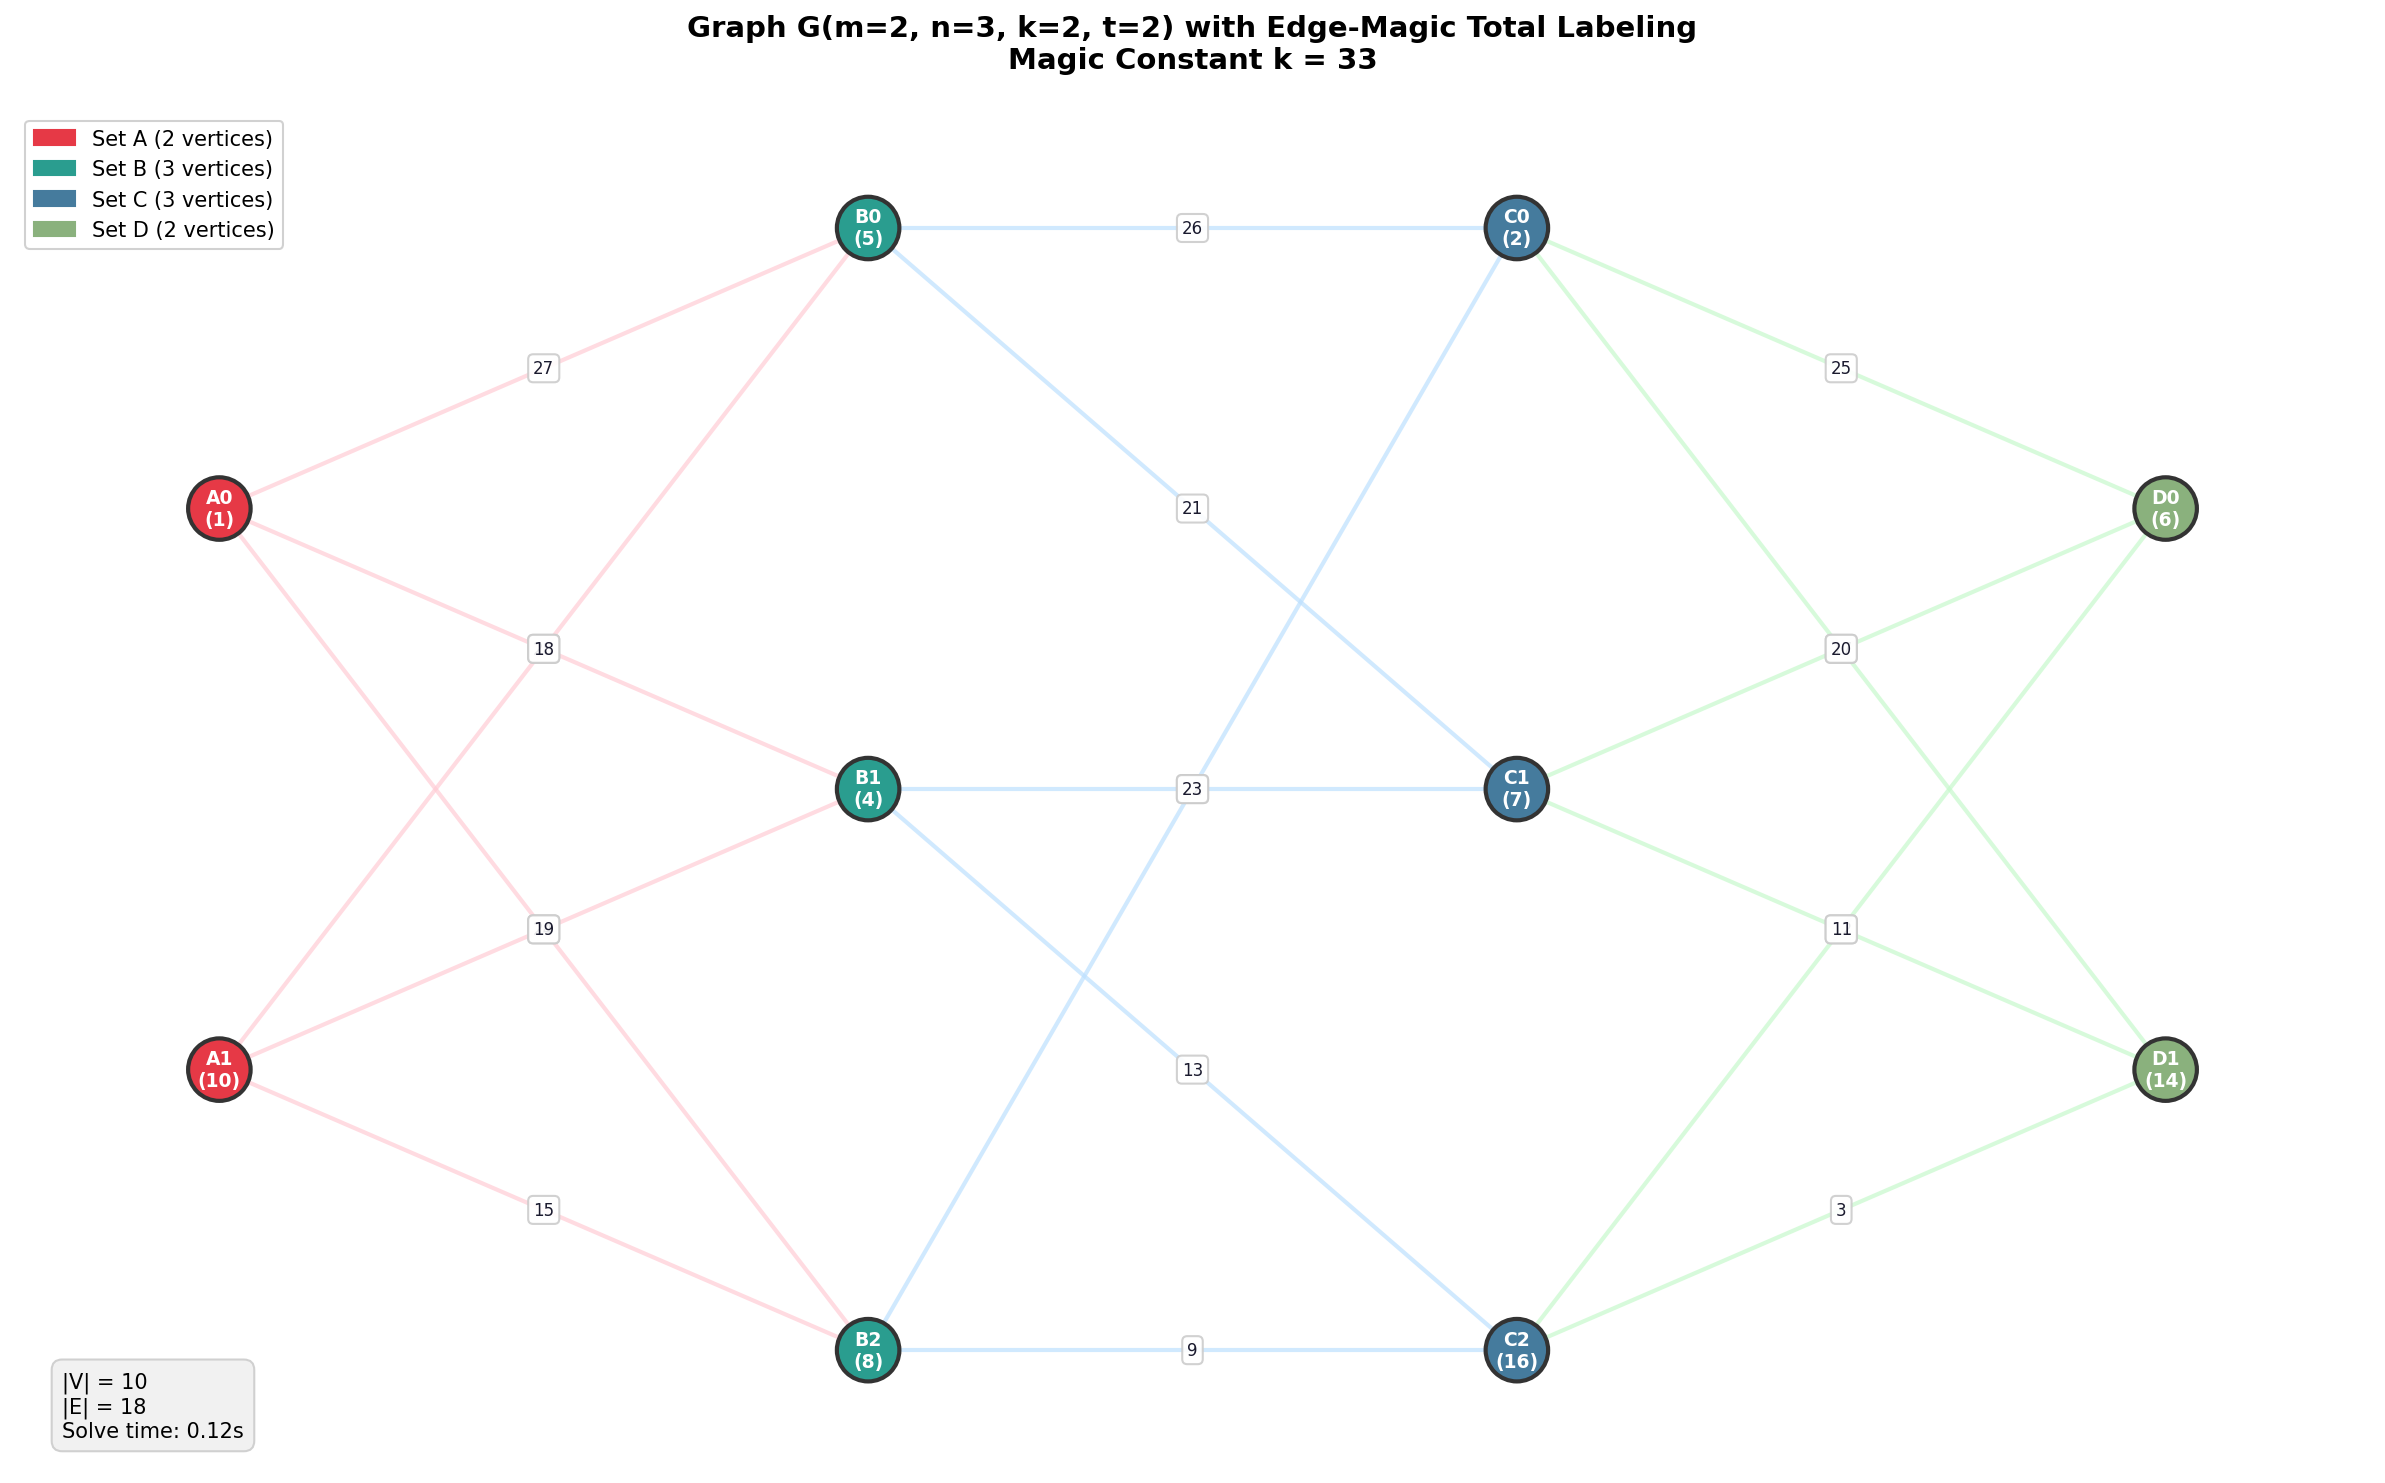
\includegraphics[width=\textwidth]{emtl_m2_n3_k2_t2.png}
    \subcaption{$G(2,3,2,2)$}
  \end{minipage}\hfill
  \begin{minipage}{0.49\textwidth}
    \centering
    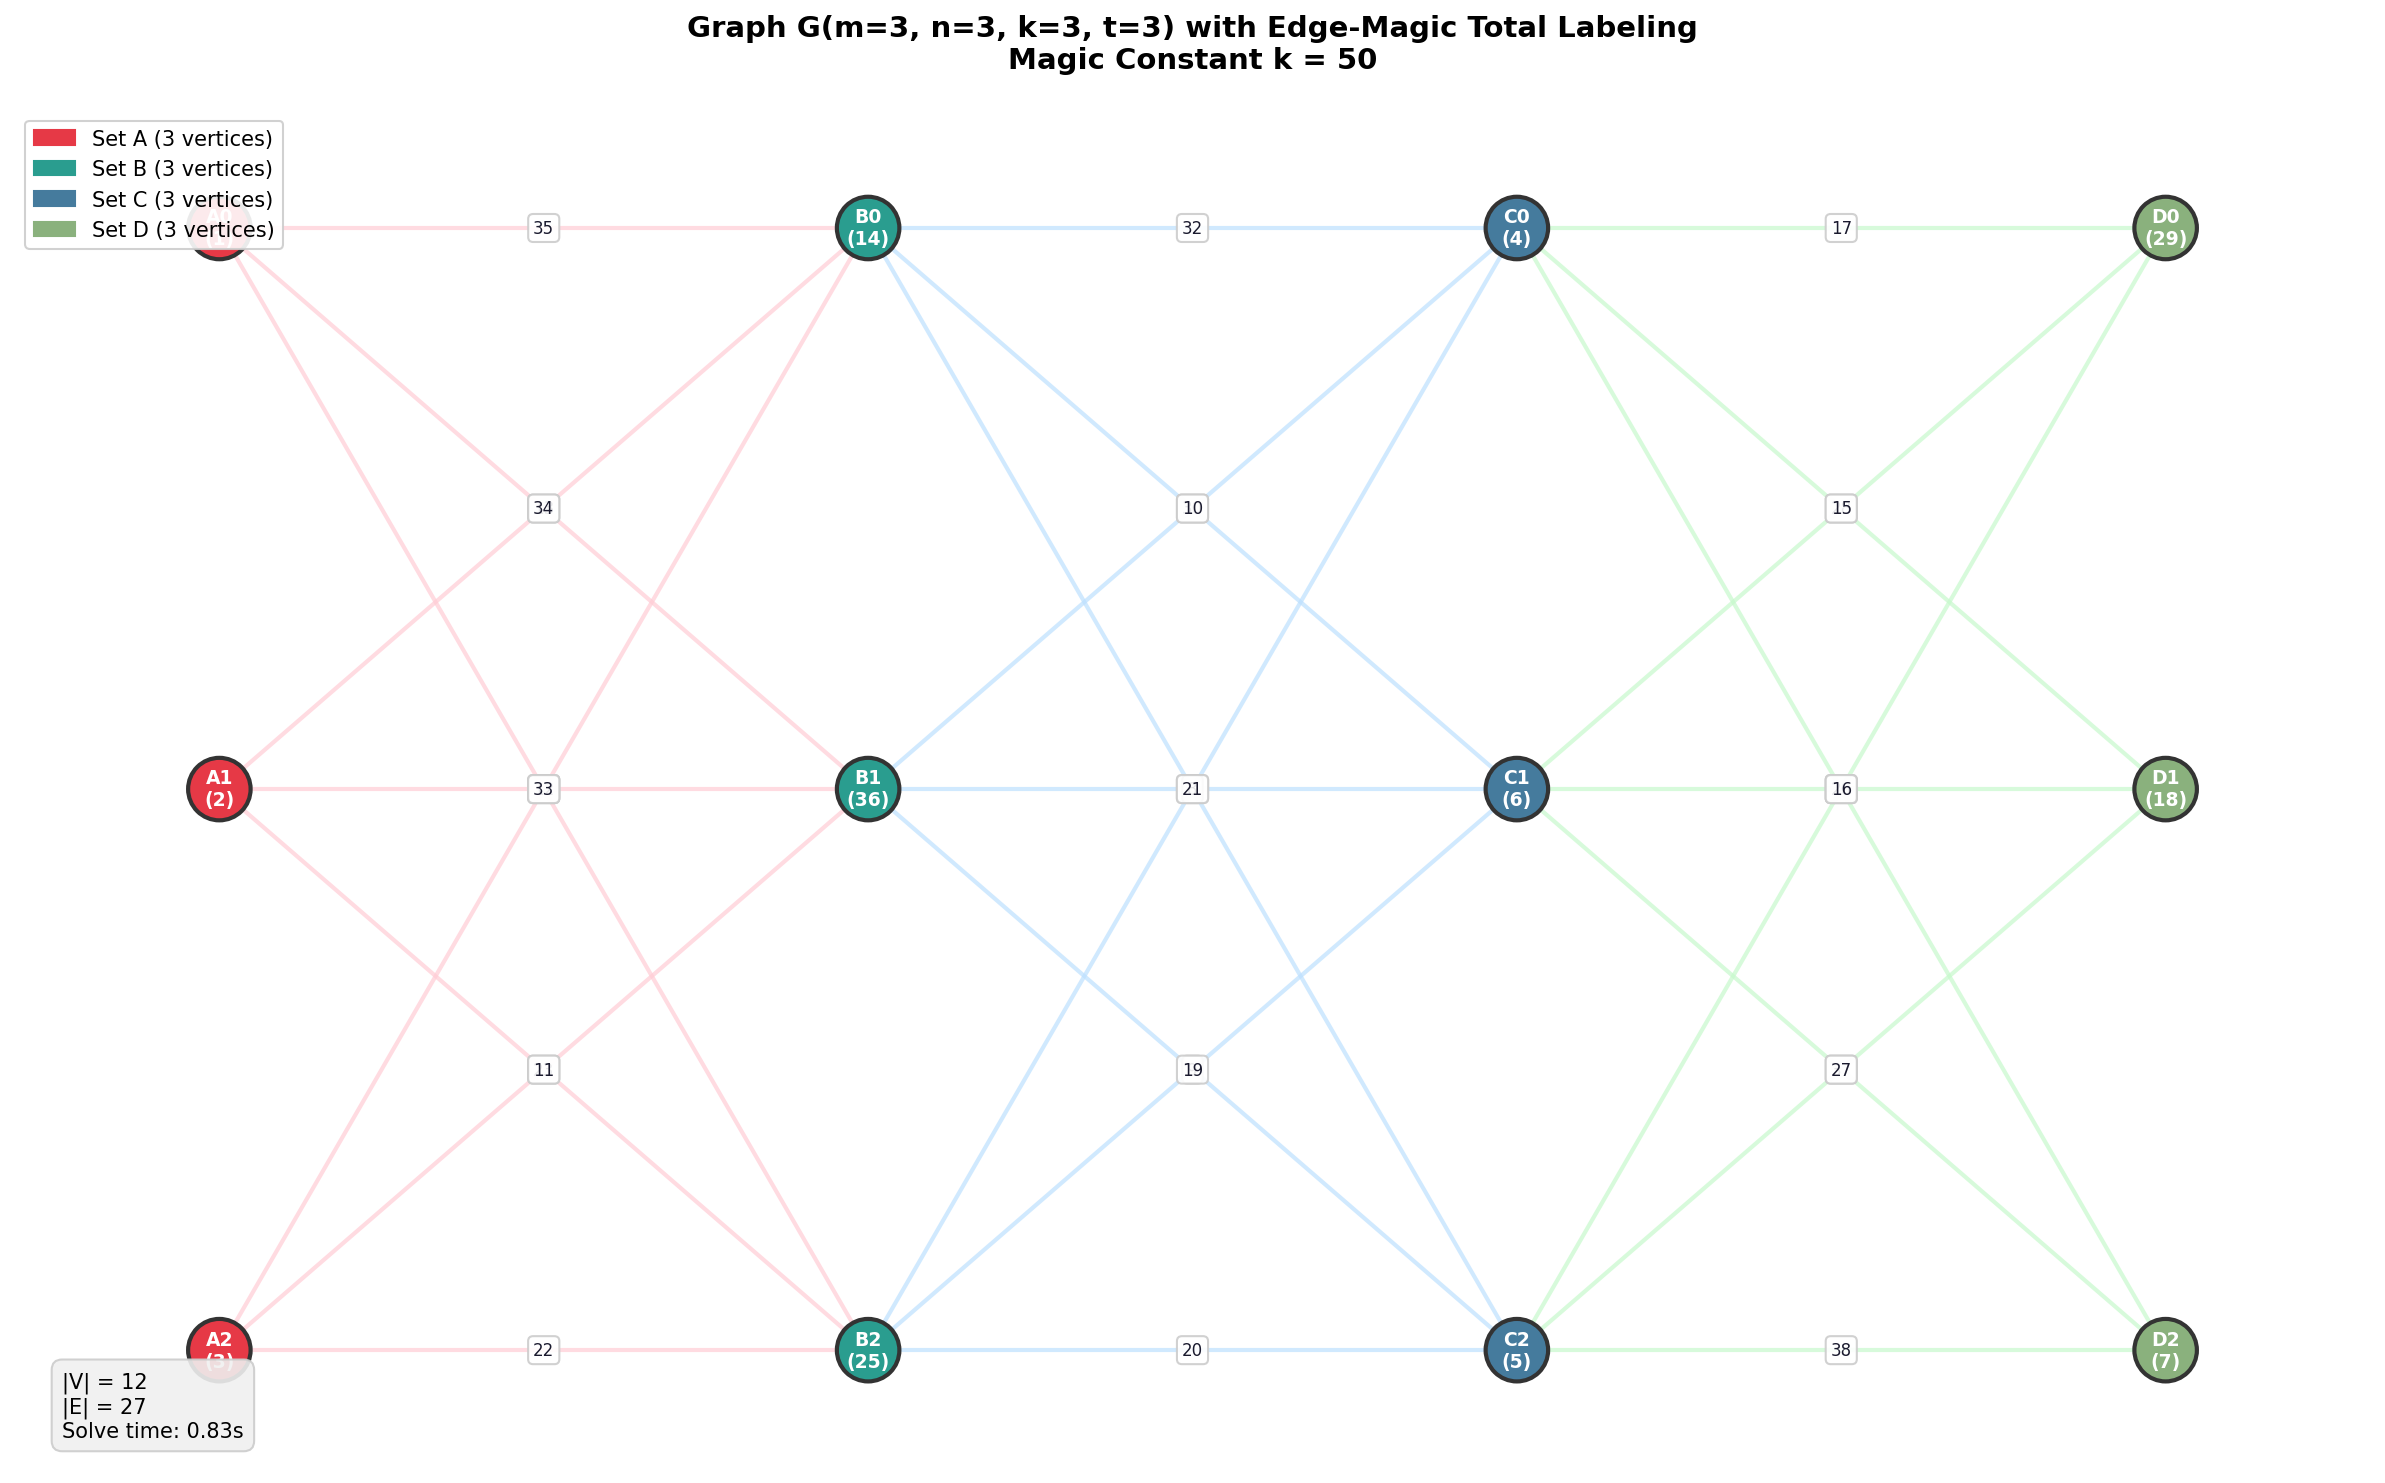
\includegraphics[width=\textwidth]{emtl_m3_n3_k3_t3.png}
    \subcaption{$G(3,3,3,3)$}
  \end{minipage}
  \caption{برچسب‌گذاری‌های جادویی کلِ یالِ محاسبه‌شده برای دو عضوِ بزرگ‌ترِ خانواده.
  بخش‌ها از چپ به راست با $A,B,C,D$ رنگ‌آمیزی شده‌اند؛ هر برچسبِ یال برابرِ ثابت جادویی
  منهای دو برچسبِ سرهای آن است.}
  \label{fig:examples}
\end{figure}

\section{نتیجه‌گیری}\label{sec:conclusion}

ما برچسب‌گذاری‌های جادویی کلِ یال‌ها را روی یک خانوادهٔ ساختارمندِ چهاربخشیِ $\Gfam$
مطالعه کردیم. یک اتحادِ وزن‌دار بر حسبِ درجه، یک شرطِ بخش‌پذیری و کران‌هایی برای ثابت
جادویی استخراج کردیم و یک تحویلِ تعیین‌شدگی توسط رأس‌ها را اثبات نمودیم که به‌محضِ
تثبیتِ برچسبِ رأس‌ها و $\km$، برچسب‌گذاری را مشخص می‌کند. بیانِ وجود به‌صورتِ یک مسئلهٔ
ارضای قیود و حلِ آن با \en{CP-SAT}، روشی دقیق به‌دست می‌دهد که یک برچسب‌گذاریِ
تأییدشده، یک اثباتِ ناممکن‌بودن، یا اعلامِ اتمامِ زمان بازمی‌گرداند. گام‌های طبیعیِ بعدی
عبارت‌اند از مشخص‌کردنِ نواحیِ پارامتری که در آن‌ها $\Gfam$ یال‌جادویی است، افزودنِ
قیدهای شکستنِ تقارن با بهره‌گیری از ساختارِ دوریِ لایهٔ میانی، و سوق‌دادنِ حل‌کننده به
سمتِ نمونه‌های بزرگ‌تر.

\paragraph{دسترسی.}
کدِ منبع، مجموعه‌آزمون، ابزارِ ترسیم و این مقاله در مخزنِ پروژه در دسترس‌اند.

\begin{thebibliography}{9}
\setLTR\enfont
\bibitem{kotzig-rosa}
  A.~Kotzig and A.~Rosa,
  \emph{Magic valuations of finite graphs},
  Canad. Math. Bull. \textbf{13} (1970), 451--461.

\bibitem{wbms}
  W.~D.~Wallis, E.~T.~Baskoro, M.~Miller, and Slamin,
  \emph{Edge-magic total labelings},
  Australas. J. Combin. \textbf{22} (2000), 177--190.

\bibitem{wallis}
  W.~D.~Wallis,
  \emph{Magic Graphs},
  Birkh\"auser, Boston, 2001.

\bibitem{gallian}
  J.~A.~Gallian,
  \emph{A dynamic survey of graph labeling},
  Electron. J. Combin., Dynamic Survey \#DS6.

\bibitem{kite}
  I.~Singgih,
  \emph{Edge magic total labeling of $(n,t)$-kites},
  in Proc.\ Int.\ Conf.\ on Mathematics, Geometry, Statistics, and Computation
  (IC-MaGeStiC 2021), Atlantis Press, 2022, pp.\ 26--31.
  \url{https://www.atlantis-press.com/proceedings/ic-magestic-21/125970045}.

\bibitem{ortools}
  Google,
  \emph{OR-Tools CP-SAT solver} (documentation).
  \url{https://developers.google.com/optimization/cp/cp_solver}.
\end{thebibliography}

\end{document}
